% vim:ft=tex

\section{2-digits Distance Database}

\subsection{Algorithm}

If we computed the distance between all cities in Europe, it would take a very
long time and file the hard drive consequently.
To reduce the effort was decided to group each postcode by its region (most of the
time represented by the two first digits). Then we compute the distance ``as the
crow flies'' and by road between each of these regions and store them into the database.

When requesting the distance between two postcode, we process as such:
\begin{enumerate}
  \item transform both postcode into coordinates
  \item calculate the distance as the crow flies (named $d_{direct,crow}$)
  \item determine the two 2-digit regions associated
  \item get the distance ``as the crow flies'' ($d_{region,crow}$) and by road
      ($d_{region,road}$) between the two regions from the database
  \item calculate the ratio $ratio = d_{region,road}/d_{region,crow}$
  \item the final distance estimate is $d_{direct,crow} * ratio$
\end{enumerate}

The calculation is summarized by figure~\ref{fig:calc}.
\begin{figure}[H]
\centering
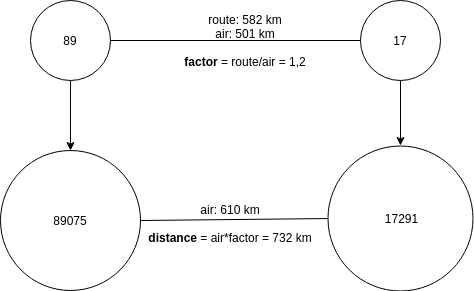
\includegraphics[width=0.7\textwidth]{img/calc}
\captionof{figure}{Theoretical example of distance calculation}\label{fig:calc}
\end{figure}
